\documentclass{article}
\usepackage{amsmath,amssymb}
\usepackage{hyperref}
\usepackage{graphicx}
\usepackage{todonotes}

\title{\bf{Laboratory Project Two: Calibration of an Orifice Meter}}
\author{Nicholas Malaya \\ Department of Mechanical Engineering \\
University of Texas at Austin} \date{} 

\begin{document}
\maketitle
\date{}
\newpage
\section{Objectives}

\textbf{A short paragraph listing the specific objectives of this laboratory.}   


\section{Background and Experimental Details}

\textbf{Describe the basic operation of an LDV. Explain what frequency
shifting is, and why it is used. Calculate the following: 
\begin{itemize}
 \item Size of the Probe Volume
 \item Expected frequency response of the glass sphere seed particles
\end{itemize}
}   

  % \begin{figure}[!htb]
  %  \begin{center}
  %   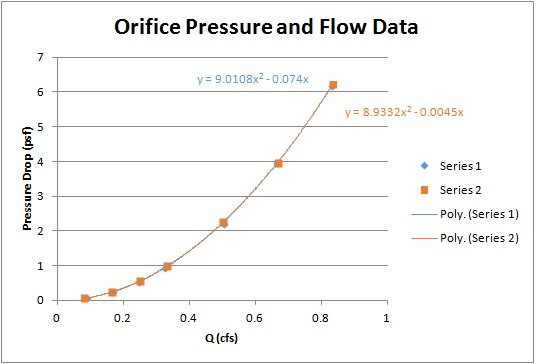
\includegraphics[width = 12 cm]{figs/Q_dP_fits.jpg}
  %   \caption{A plot of repeatability of the experiment. }
  %   \label{orif-zoom}
  %  \end{center}
  % \end{figure}

\section{Experiment One: Freestream}

\textbf{Indicate the frequency shift and bandpass filter settings used,
and why} 

\section{Experiment Two: Wake Measurements}

\textbf{Present results from your wake measurements, including
uncertainty of the measurements. Compare your results with data in the
literature and comment on similarities and differences. } 


\section{Conclusions}


\textbf{Conclude by giving your opinion about whether your measurements
are more or less reliable than measurements in the literature.} 

%
%
%
\end{document}

% LocalWords:  reynolds H20 piecewise RDG yar
